\subsection{Validazione e collaudo}

\subsubsection{IX Incremento}
\subsubsubsection{Prospetto orario}
In questo incremento la distribuzione oraria è la seguente:
\begin{table}[H]
\begin{center}
\rowcolors{2}{gray!25}{white}
\renewcommand{\arraystretch}{1.25}
\begin{tabular}{ m{0.20\textwidth}<{\centering}  m{0.06\textwidth}<{\centering} m{0.06\textwidth}<{\centering} m{0.06\textwidth}<{\centering}  m{0.06\textwidth}<{\centering}  m{0.06\textwidth}<{\centering}  m{0.06\textwidth}<{\centering}  m{0.20\textwidth}<{\centering}   }
	\rowcolor{darkblue}
	\textcolor{white}{\textbf{Componente}} &\textcolor{white}{\textbf{Re}}&\textcolor{white}{\textbf{Pt}}&\textcolor{white}{\textbf{An}}&\textcolor{white}{\textbf{Am}}&\textcolor{white}{\textbf{Pr}}&\textcolor{white}{\textbf{Ve}}&\textcolor{white}{\textbf{Ore complessive}}\\ 
	Edoardo Pavan & 1 & 0 & 0 & 0 & 6 & 2 & 9 \\	
	
	Francesco Protopapa & 2 & 0 & 0 & 2 & 5 & 3 & 12 \\

	Greta Cavedon & 1 & 1 & 0 & 2 & 3 & 3 & 10 \\
	
	Luciano Wu & 0 & 4 & 0 & 0 & 5 & 2 & 11 \\
	
	Matteo Basso & 0 & 1 & 0 & 2 & 2 & 1 & 6 \\
	
	Michele Gatto & 2 & 2 & 0 & 0 & 4 & 1 & 9 \\
	
	Pietro Villatora & 1 & 3 & 0 & 0 & 4 & 1 & 9 \\
	
	\textbf{Ore totali ruolo} & 7 & 11 & 0 & 6 & 29 & 13 & 66 \\

\end{tabular}
\caption{Distribuzione oraria per ogni componente nel IX incremento, Validazione e Collaudo}
\end{center}
\end{table}

La tabella può essere rappresentata anche in forma visiva dal seguente grafico:
\begin{figure}[H]
\centering
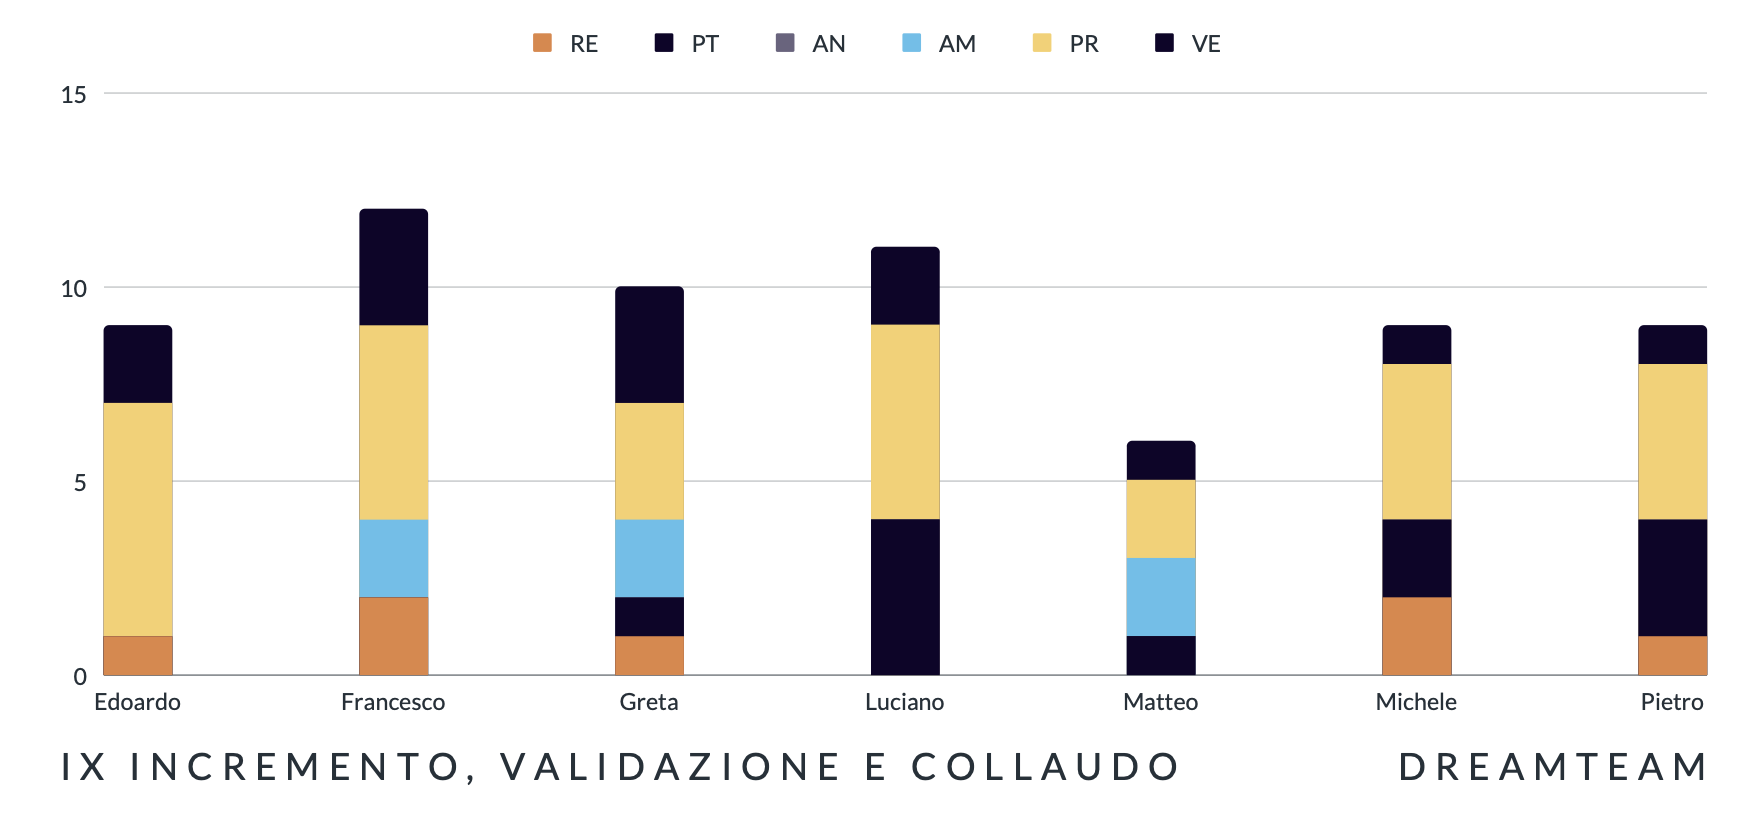
\includegraphics[scale=0.55]{Sezioni/SezioniPreventivo/grafici/Preventivo_validazione_collaudo_IX.png}
\caption{Istogramma della ripartizione delle ore nel IX incremento, Validazione e Collaudo}
\end{figure}

\subsubsubsection{Prospetto economico}
La seguente tabella rappresenta le ore totali dedicate ad ogni ruolo e il costo in euro:

\begin{table}[H]
\begin{center}
\rowcolors{2}{gray!25}{white}
\renewcommand{\arraystretch}{1.5}
\begin{tabular}{ m{0.3\textwidth}<{\centering}  m{0.2\textwidth}<{\centering} m{0.2\textwidth}<{\centering}}
	\rowcolor{darkblue}
	\textcolor{white}{\textbf{Ruolo}}&\textcolor{white}{\textbf{Totale ore}}&\textcolor{white}{\textbf{Costo totale (\euro)}}\\ 

	Responsabile  & 7 & 210 \\	
	
	Progettista & 11 & 220 \\
	
	Analista & 0 & 0 \\

	Amministratore & 6 & 150 \\
	
	Programmatore & 29 & 435 \\
	
	Verificatore & 13 & 195 \\
	
	\textbf{Totale} & 66 & 1210 \\
	
\end{tabular}
\caption{Prospetto dei costi per ruolo nel IX incremento, Validazione e Collaudo}
\end{center}
\end{table}

La tabella può essere rappresentata anche in forma visiva dal seguente aerogramma:
\begin{figure}[H]
\centering
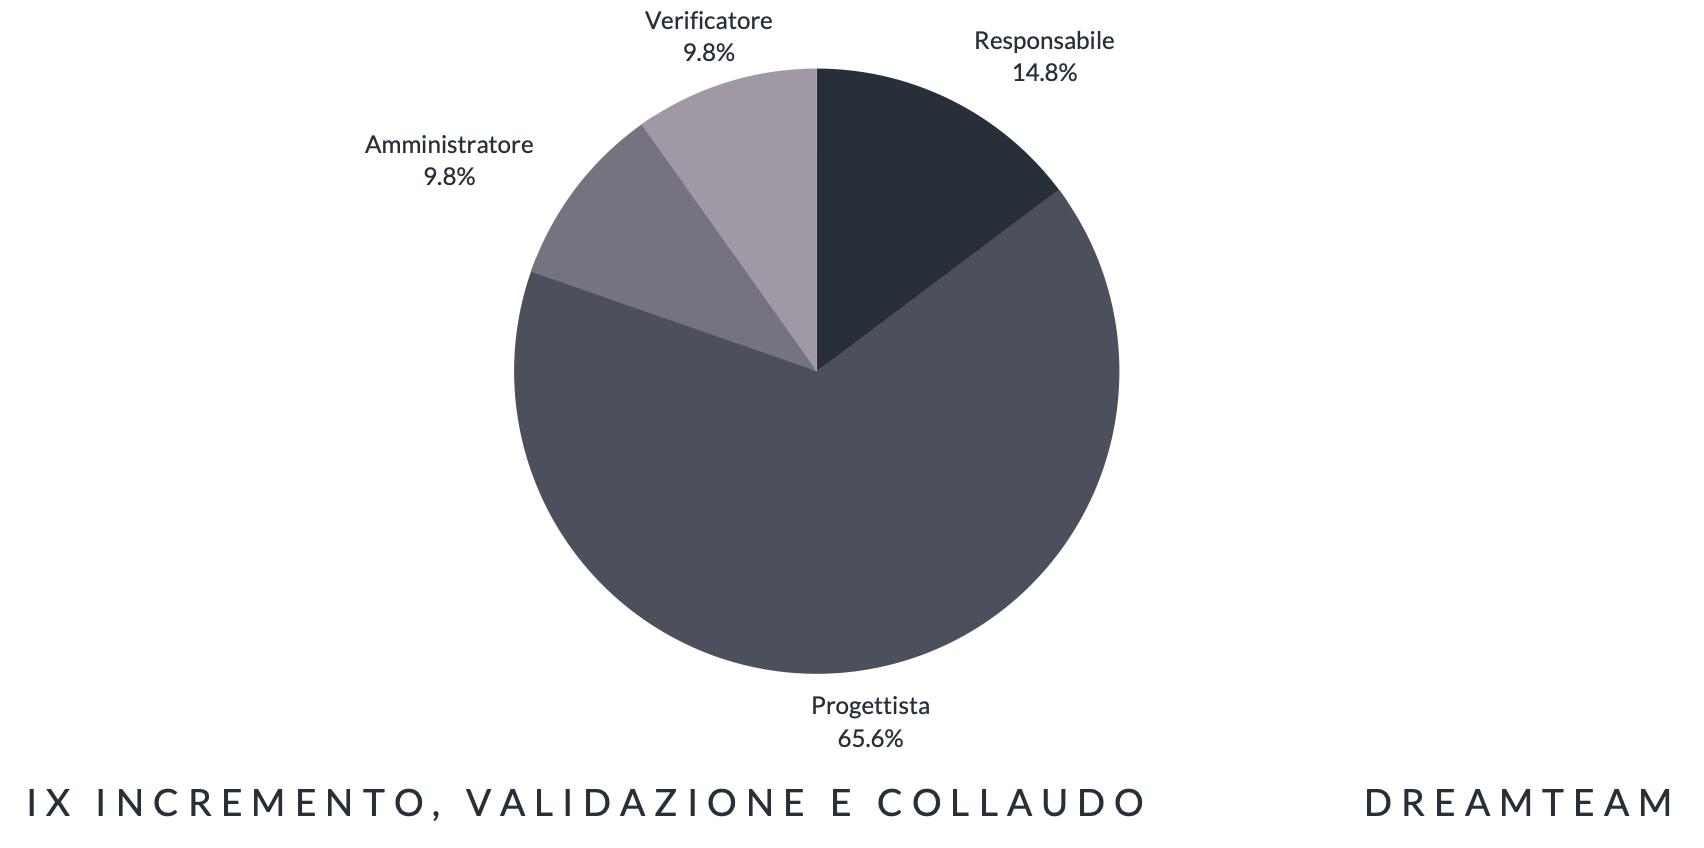
\includegraphics[scale=0.55]{Sezioni/SezioniPreventivo/grafici/Preventivo_torta_validazione_collaudo_IX.png}
\caption{Grafico a torta della ripartizione per ruolo delle ore durante il IX incremento, Validazione e Collaudo}
\end{figure}

\pagebreak

\subsubsection{X Incremento}
\subsubsubsection{Prospetto orario}
In questo incremento la distribuzione oraria è la seguente:
\begin{table}[H]
\begin{center}
\rowcolors{2}{gray!25}{white}
\renewcommand{\arraystretch}{1.25}
\begin{tabular}{ m{0.20\textwidth}<{\centering}  m{0.06\textwidth}<{\centering} m{0.06\textwidth}<{\centering} m{0.06\textwidth}<{\centering}  m{0.06\textwidth}<{\centering}  m{0.06\textwidth}<{\centering}  m{0.06\textwidth}<{\centering}  m{0.20\textwidth}<{\centering}   }
	\rowcolor{darkblue}
	\textcolor{white}{\textbf{Componente}} &\textcolor{white}{\textbf{Re}}&\textcolor{white}{\textbf{Pt}}&\textcolor{white}{\textbf{An}}&\textcolor{white}{\textbf{Am}}&\textcolor{white}{\textbf{Pr}}&\textcolor{white}{\textbf{Ve}}&\textcolor{white}{\textbf{Ore complessive}}\\ 
	Edoardo Pavan & 1 & 0 & 0 & 0 & 4 & 2 & 7 \\	
	
	Francesco Protopapa & 1 & 0 & 0 & 2 & 4 & 1 & 8 \\

	Greta Cavedon & 2 & 0 & 0 & 2 & 3 & 4 & 11 \\
	
	Luciano Wu & 0 & 3 & 0 & 0 & 5 & 1 & 9 \\
	
	Matteo Basso & 0 & 1 & 0 & 2 & 2 & 3 & 8 \\
	
	Michele Gatto & 1 & 3 & 0 & 0 & 2 & 2 & 8 \\
	
	Pietro Villatora & 2 & 2 & 0 & 0 & 3 & 1 & 8 \\
	
	\textbf{Ore totali ruolo} & 7 & 9 & 0 & 6 & 23 & 15 & 60 \\

\end{tabular}
\caption{Distribuzione oraria per ogni componente nel X incremento, Validazione e Collaudo}
\end{center}
\end{table}

La tabella può essere rappresentata anche in forma visiva dal seguente grafico:
\begin{figure}[H]
\centering
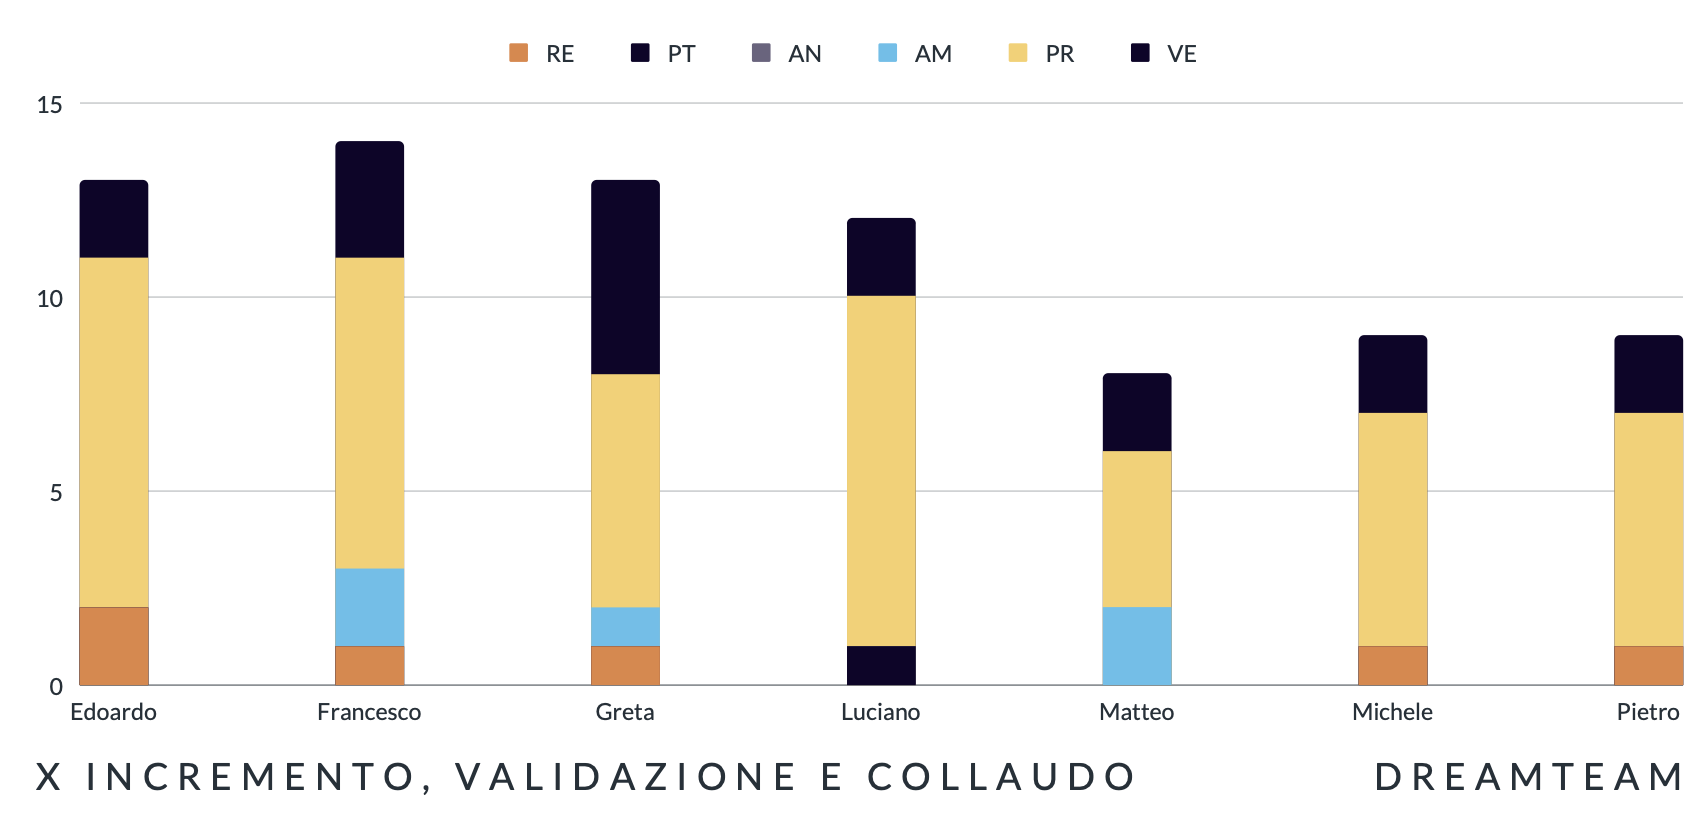
\includegraphics[scale=0.55]{Sezioni/SezioniPreventivo/grafici/Preventivo_validazione_collaudo_X.png}
\caption{Istogramma della ripartizione delle ore nel X incremento, Validazione e Collaudo}
\end{figure}

\subsubsubsection{Prospetto economico}
La seguente tabella rappresenta le ore totali dedicate ad ogni ruolo e il costo in euro:

\begin{table}[H]
\begin{center}
\rowcolors{2}{gray!25}{white}
\renewcommand{\arraystretch}{1.5}
\begin{tabular}{ m{0.3\textwidth}<{\centering}  m{0.2\textwidth}<{\centering} m{0.2\textwidth}<{\centering}}
	\rowcolor{darkblue}
	\textcolor{white}{\textbf{Ruolo}}&\textcolor{white}{\textbf{Totale ore}}&\textcolor{white}{\textbf{Costo totale (\euro)}}\\ 

	Responsabile  & 7 & 210 \\	
	
	Progettista & 9 & 180 \\
	
	Analista & 0 & 0 \\

	Amministratore & 6 & 150 \\
	
	Programmatore & 23 & 345 \\
	
	Verificatore & 15 & 225 \\
	
	\textbf{Totale} & 60 & 1110 \\
	
\end{tabular}
\caption{Prospetto dei costi per ruolo nel X incremento, Validazione e Collaudo}
\end{center}
\end{table}

La tabella può essere rappresentata anche in forma visiva dal seguente aerogramma:
\begin{figure}[H]
\centering
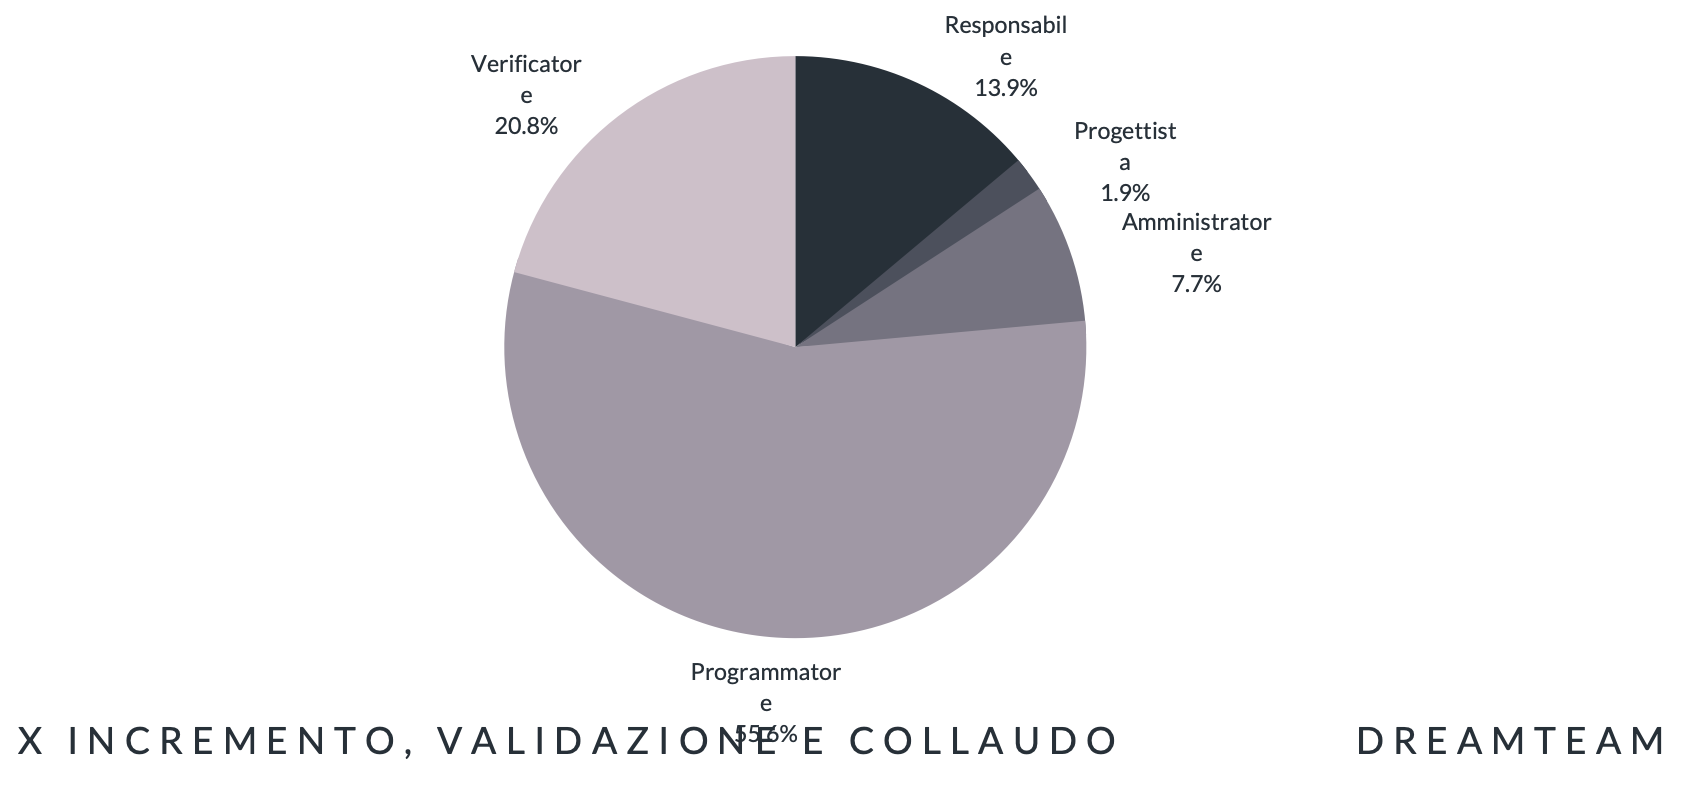
\includegraphics[scale=0.55]{Sezioni/SezioniPreventivo/grafici/Preventivo_torta_validazione_collaudo_X.png}
\caption{Grafico a torta della ripartizione per ruolo delle ore durante il X incremento, Validazione e Collaudo}
\end{figure}

\pagebreak

\subsubsection{Fase complessiva}
\subsubsubsection{Prospetto orario}
La seguente tabella rappresenta la distribuzione oraria per ogni componente del gruppo nella fase di Validazione e Collaudo:
\begin{table}[H]
\begin{center}
\rowcolors{2}{gray!25}{white}
\renewcommand{\arraystretch}{1.25}
\begin{tabular}{ m{0.20\textwidth}<{\centering}  m{0.06\textwidth}<{\centering} m{0.06\textwidth}<{\centering} m{0.06\textwidth}<{\centering}  m{0.06\textwidth}<{\centering}  m{0.06\textwidth}<{\centering}  m{0.06\textwidth}<{\centering}  m{0.20\textwidth}<{\centering}   }
	\rowcolor{darkblue}
	\textcolor{white}{\textbf{Componente}} &\textcolor{white}{\textbf{Re}}&\textcolor{white}{\textbf{Pt}}&\textcolor{white}{\textbf{An}}&\textcolor{white}{\textbf{Am}}&\textcolor{white}{\textbf{Pr}}&\textcolor{white}{\textbf{Ve}}&\textcolor{white}{\textbf{Ore complessive}}\\ 
	Edoardo Pavan & 2 & 0 & 0 & 0 & 10 & 4 & 16 \\	
	
	Francesco Protopapa & 3 & 0 & 0 & 4 & 9 & 5 & 21 \\

	Greta Cavedon & 3 & 1 & 0 & 4 & 6 & 7 & 21 \\
	
	Luciano Wu & 0 & 7 & 0 & 0 & 10 & 3 & 20 \\
	
	Matteo Basso & 0 & 2 & 0 & 4 & 4 & 4 & 14 \\
	
	Michele Gatto & 3 & 5 & 0 & 0 & 6 & 3 & 17 \\
	
	Pietro Villatora & 3 & 5 & 0 & 0 & 7 & 2 & 17 \\
	
	\textbf{Ore totali ruolo} & 14 & 20 & 0 & 12 & 52 & 28 & 126\\

\end{tabular}
\caption{Distribuzione oraria per ogni componente nella fase di Validazione e Collaudo}
\end{center}
\end{table}

La tabella può essere rappresentata anche in forma visiva dal seguente grafico:
\begin{figure}[H]
\centering
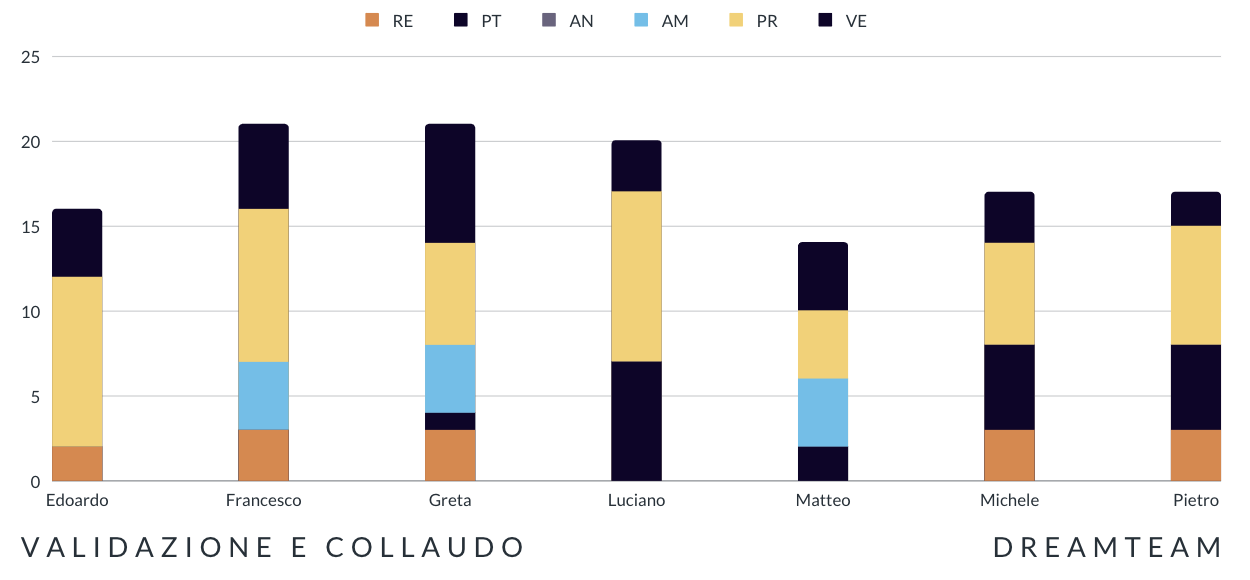
\includegraphics[scale=0.65]{Sezioni/SezioniPreventivo/grafici/Validazione_collaudo.png}
\caption{Istogramma della ripartizione delle ore nella fase di Validazione e Collaudo}
\end{figure}

\subsubsubsection{Prospetto economico}
La seguente tabella rappresenta le ore totali dedicate ad ogni ruolo e il costo in euro:

\begin{table}[H]
\begin{center}
\rowcolors{2}{gray!25}{white}
\renewcommand{\arraystretch}{1.5}
\begin{tabular}{ m{0.3\textwidth}<{\centering}  m{0.2\textwidth}<{\centering} m{0.2\textwidth}<{\centering}}
	\rowcolor{darkblue}
	\textcolor{white}{\textbf{Ruolo}}&\textcolor{white}{\textbf{Totale ore}}&\textcolor{white}{\textbf{Costo totale (\euro)}}\\ 

	Responsabile  & 14 & 420 \\	
	
	Progettista & 20 & 500 \\
	
	Analista & 0 & 0 \\

	Amministratore & 12 & 240 \\
	
	Programmatore & 52 & 780 \\
	
	Verificatore & 28 & 420 \\
	
	\textbf{Totale} & 126 & 2360 \\
	
\end{tabular}
\caption{Prospetto dei costi per ruolo nella fase di Validazione e Collaudo}
\end{center}
\end{table}

La tabella può essere rappresentata anche in forma visiva dal seguente aerogramma:
\begin{figure}[H]
\centering
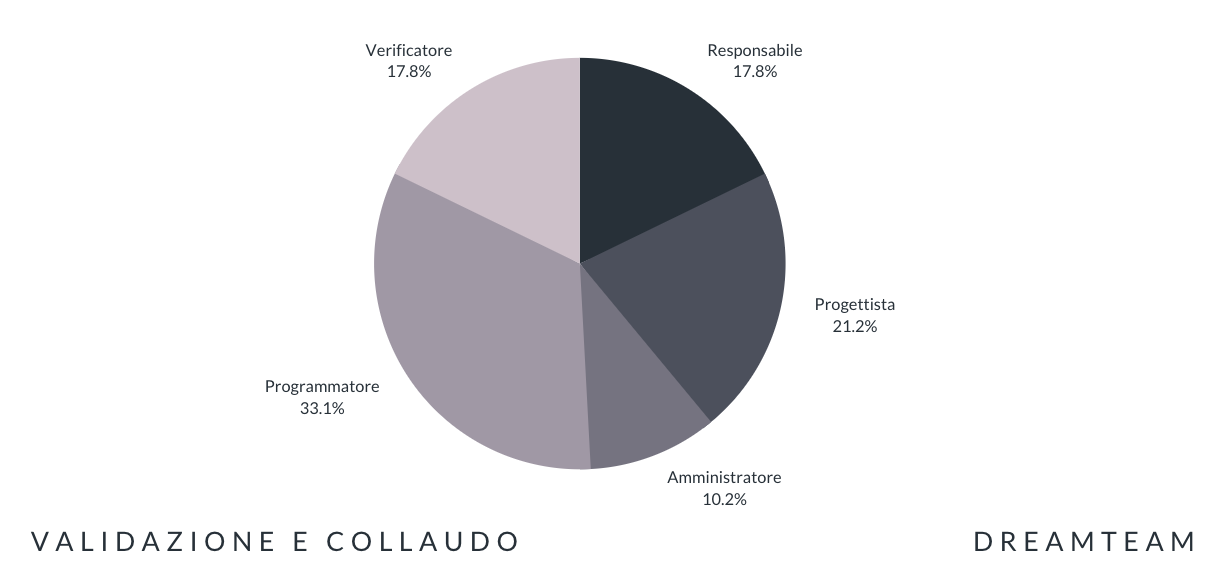
\includegraphics[scale=0.65]{Sezioni/SezioniPreventivo/grafici/Validazione_costi.png}
\caption{Grafico a torta della ripartizione per ruolo delle ore durante la fase di Validazione e Collaudo}
\end{figure}
